\documentclass[ignorenonframetext,11pt]{beamer}
%\usepackage[ngerman]{babel}
\usepackage[T1]{fontenc}
\usepackage[utf8]{inputenc}
\usepackage{lmodern}
\usepackage{tcolorbox}
\usepackage{amsmath,amssymb,amsfonts}

\usetheme{default}
%  \usecolortheme{crane}
\setbeamercovered{transparent}
%  \setlength{\parindent}{0pt}
%  \setlength{\parskip}{1.35ex plus 0.5ex minus 0.3ex}
%  \usefonttheme{structuresmallcapsserif}
\usefonttheme{structurebold}
\setbeamertemplate{theorems}[numbered]
\setbeamertemplate{sidebar right}{}
\usepackage{amscd}

\usepackage{tikz}
\usepackage{pgfplots,adjustbox}
\usepackage{eurosym}
\usepackage{graphicx}
\graphicspath{{.}{figures/}}
\usepackage{multimedia}
\usepackage{psfrag}
\usepackage{listings}

\lstset{language=C++, basicstyle=\small\ttfamily,
  keywordstyle=\bfseries, tabsize=4, stringstyle=\ttfamily,morekeywords={decltype},
  extendedchars=true, escapeinside={/*@}{@*/}}
\definecolor{darkgray}{gray}{0.4}
\lstset{keywordstyle=\color{green!40!black},
  commentstyle=\itshape\color{blue!30!black!40!white},
  stringstyle=\color{blue!60!black!60!white},
  emph={bool,int,unsigned,char,true,false,void}, emphstyle=\color{red!80!black},
  emph={[2]\#include,\#define,\#ifdef,\#endif}, emphstyle={[2]\color{green!60!black}},
  emph={[3]Dune,Grid,SomeGrid,TheGrid,LeafIterator,LevelIterator,LeafIntersectionIterator,LevelIntersectionIterator,Geometry,GeometryType,QuadraturePoint,QuadratureRule,PDELab,Entity,EntityPointer,Codim,FieldVector,FieldMatrix}, emphstyle={[3]\color{blue!60!black}}
}
\usepackage{curves}
%\usepackage{epic}
\usepackage{calc}
%\usepackage{picinpar}
%\usepackage{fancybox}
%\usepackage{xspace}
\usepackage{enumerate}
\usepackage{algpseudocode}
\usepackage{color}
\usepackage{bold-extra}
\usepackage{bm}
\usepackage{stmaryrd}
%\usepackage[squaren]{SIunits}
\usepackage{nicefrac}

\usepackage{fancyvrb,bbm,xspace}
\usepackage{lmodern}
\usepackage{fancyvrb,bbm,xspace}
\usepackage[binary-units]{siunitx}
\usepackage{xcolor,tabu}

\definecolor{niceblue}{rgb}{0.122,0.396,0.651}   %% 31, 101, 166 or #1F65A6
\definecolor{niceorange}{RGB}{255,205,86}        %% #FFCD56
\definecolor{nicered}{RGB}{220,20,60}                      %% rgb(220, 20, 60)
\definecolor{niceteal}{HTML}{00A9AB}
\definecolor{niceviolet}{HTML}{820080}

\def\clap#1{\hbox to 0pt{\hss#1\hss}}
\definecolor{dunedarkblue}{rgb}{0.22, 0.29, 0.49}
\definecolor{dunemediumblue}{rgb}{0.35, 0.45, 0.71}
\definecolor{dunelightblue}{rgb}{0.61, 0.68, 0.85}
\definecolor{duneorange}{rgb}{0.91, 0.56, 0.25}

\definecolor{niceblueLight}{HTML}{91CAFB}
\definecolor{niceblueVeryLight}{HTML}{DDEFFF}

\usepackage{lmodern}
\usepackage{inconsolata}
\usepackage{nimbusmononarrow}
%\renewcommand*\ttdefault{txtt}
\usepackage{dsfont}

\theoremstyle{definition}

\title{Simulation Workflow - Build system, meshes and visualization}
\author{Dominic Kempf}

\begin{document}

\begin{frame}
\titlepage
\end{frame}

\begin{frame}
 \frametitle{Goals of this lecture}

 At the end of this lecture/exercise session you should
 \begin{itemize}
  \item understand the modular structure of Dune.
  \item have realized that build systems are your friend!
  \item have an overview of available grid implementations in Dune
  \item have seen several concepts to construct grids
  \item be able to visualize PDE solutions in ParaView
 \end{itemize}

\end{frame}


\section{Modular structure of Dune}

\begin{frame}[fragile]
 Dune is distributed as a zoo of projects.
 They fall into the following categories:

 \begin{itemize}
  \item \textit{core modules}: Basic infrastructure and data types,
  Grid interface, geometries, basis functions and linear algebra
  \item \textit{discretization modules}: \textbf{dune-pdelab},
  dune-fem, dune-fufem, ...
  \item \textit{Grid modules}: Additional grid managers
  \item \textit{Extension modules}: Mixed bag of additional functionalities
  \item \textit{User modules}
 \end{itemize}

 Each module...
 \begin{itemize}
  \item is a git repository in itself
  \item has a file \textit{dune.module}, which describes its dependencies
  \item uses the build system from dune-common
 \end{itemize}

 New modules are created with a shell script \lstinline!duneproject!
\end{frame}


\section{Build system}


\begin{frame}[fragile]
 \frametitle{What is CMake anyway?}
 CMake...
 \begin{itemize}
  \item ... is an open source buildsystem tool developed at KITware.
  \item ... offers a one-tool-solution to all building tasks, like configuring, building, linking, testing and packaging.
  \item ... is a build system generator: It supports a set of backends called ``generators''
  \item ... is portable
  \item ... is controlled by ONE rather simple language
 \end{itemize}
 \vspace{0.5cm}
 We typically use the \lstinline!Unix Makefiles! generator that generates Makefiles.
\end{frame}

\begin{frame}[fragile]
 \frametitle{Where is the build system defined?}
 Each (sub)directory of the project contains a file \lstinline!CMakeLists.txt!. This file
 \begin{itemize}
  \item is written in the CMake language
  \item is run during configure
  \item recursively runs \lstinline!CMakeLists.txt! files from subdirectories.
 \end{itemize}
\end{frame}

\begin{frame}[fragile]
 \frametitle{Some CMake commands everybody should know}

 \begin{itemize}
  \item \lstinline!add_subdirectory! lets the configure script recurse into a subdirectory.
  A \lstinline!CMakeLists.txt! file is expected in that directory.
  \item \lstinline!add_executable! adds build rules for a new executable.
  \item \lstinline!dune_add_test! adds a test to the testing suite
  \item \lstinline!dune_symlink_to_source_files! creates links from the source directory into the build directory
 \end{itemize}
\end{frame}

\begin{frame}[fragile]
 \frametitle{An example CMakeLists.txt file}
 \begin{lstlisting}
add_executable(mytarget mycode.cc)
dune_symlink_to_source_files(FILES mygrid.grid)

dune_add_test(SOURCE unittest.cc
              MPI_RANKS 4)

add_subdirectory(mysubdir)
 \end{lstlisting}
\vspace{0.5cm}
  For a reference of end-user CMake commands, see the build system documentation on the Dune website (\textbf{DEMOTIME!}).

\end{frame}


\section{Simulation Workflow}

\begin{frame}
 \frametitle{Simulation workflow}

  \tikzstyle{materia_blue}=[draw, fill=blue!20, text width=6.0em, text centered,
  minimum height=1.5em]
  \begin{center}
 \begin{tikzpicture}[scale=0.8, transform shape]
   \path node (p1) [materia_blue, text width=6em, minimum width=6em, minimum height=3em, rounded corners]{Mesh Generation};
   \path (p1.east) + (4.0, 0.0) node (p2) [materia_blue, text width=10em, minimum width=4em, minimum height=3em, rounded corners]{Simulation Executable\\{\scriptsize\textit{Grid, Discretization, Linear Algebra}}};
   \path (p2.north) + (0.0, 2.0) node (p3) [materia_blue, text width=6em, minimum width=4em, minimum height=3em, rounded corners]{Configuration};
   \path (p2.east) + (4.0, 0.0) node (p4) [materia_blue, text width=6em, minimum width=4em, minimum height=3em, rounded corners]{Visualization};

   \draw[-latex] (p1.east) -- (p2.west);
   \draw[-latex] (p3.south) -- (p2.north);
   \draw[-latex] (p2.east) -- (p4.west);

   \path (p1.east) + (1.0, 0.2) node (p5) {\scriptsize Grid input files};
   \path (p2.east) + (1.0, 0.2) node (p6) {\scriptsize VTK file(s)};
   \path (p3.south) + (0.0, -0.5) node (p7) {\scriptsize ini file};
 \end{tikzpicture}
 \end{center}
\end{frame}

\begin{frame}[fragile]
 \frametitle{Reading configuration through ini files}
\begin{lstlisting}
outputfilename = myfile.vtu
[grid]
lowerleft = -1. -1.
upperright = 1. 1.
\end{lstlisting}
\vspace{0.5cm}
 Dune style ini files support:
 \begin{itemize}
  \item Key/value pairs separated with a \verb!=!
  \item Grouping of keys into sections to arbitrary depth
 \end{itemize}

 \begin{lstlisting}
  #include<dune/common/parametertree.hh>
  #include<dune/common/parametertreeparser.hh>

  Dune::ParameterTree tree;
  Dune::ParameterTreeParser::readINITree(filename, tree);
 \end{lstlisting}

\end{frame}

\section{Available grid implementations}

\begin{frame}
 \frametitle{Selecting a grid manager}

 Dune offers a large variety of grid managers, which differ vastly in their feature set and their natural strengths.
 Here are some capabilities of grid implementations:
 \begin{itemize}
  \item structured vs. unstructured
  \item simplical vs. quadrilateral vs. multi-geometry
  \item conforming vs. non-conforming
  \item parallel vs. sequential
  \item adaptive vs. non-adaptive (also: different refinement algorithms)
  \item different world dimensions ($1$, $2$, $3$, $n$)
  \item Surface/manifold grids
 \end{itemize}

 Dune allows for implementations of all sorts of grids through one common interface!
\end{frame}

\begin{frame}
 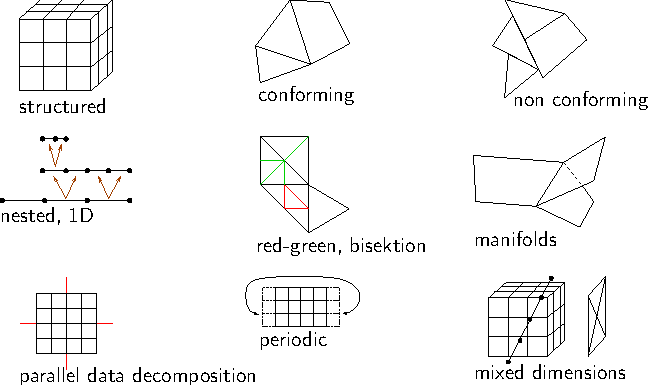
\includegraphics[width=\textwidth]{figures/io/grids.pdf}
\end{frame}


\begin{frame}
  \frametitle{A selection of available Implementations of the Dune grid interface:}
  \begin{itemize}
  \item \lstinline!YaspGrid! (in dune-grid, structured, parallel, $n$-dimensional, tensorproduct grid)
  \item \lstinline!OneDGrid! (in dune-grid, adaptive, parallel, 1D)
  \item \lstinline!GeometryGrid! (in dune-grid, meta-grid, applies discrete mesh transformation)
  \item \lstinline!dune-uggrid! (2D/3D, unstructured, parallel, multi-geometry)
  \item \lstinline!dune-alugrid! (2D/3D, unstructured, parallel, simplex/cube)
  \item \lstinline!dune-multidomaingrid! (meta-grid, partition grid into sub-domains)
  \item \lstinline!dune-subgrid! (meta-grid, part of the grid hierarchy as grid in itself)
  \item \lstinline!opm-grid! (3D, corner-point geometries)
  \item \lstinline!dune-foamgrid! (1D/2D in 3D manifold grid)
  \item \lstinline!dune-prismgrid! (meta-grid, extrudes surface mesh)
  \item \lstinline!dune-polygongrid! (polygonal geometries)
  \item \ldots{}
  \end{itemize}
\end{frame}

\section{How to create Dune grids}

\subsection{StructuredGridFactory}

\begin{frame}[fragile]
\frametitle{StructuredGridFactory}
There is a utility class, the \lstinline!StructuredGridFactory!, which makes it easy to create
structured grids (also for unstructured grid managers). It provides two static functions:
\begin{itemize}
 \item \lstinline!createCubeGrid! creates a grid with cubes with given domain size and number
of elements in each direction.
\item \lstinline!createSimplexGrid! creates a grid with simplices which are generated by subdividing
the cubes.
\end{itemize}
These return a \lstinline!unique_ptr! to a grid object.

\begin{lstlisting}[basicstyle=\scriptsize\ttfamily]
Dune::FieldVector<GridType::ctype, dim> lowerleft(0.0);
Dune::FieldVector<GridType::ctype, dim> upperright(1.0);
auto N = Dune::filledArray<dim, unsigned int>(4);

auto grid = Dune::StructuredGridFactory<GridType>::
              createCubeGrid(lowerleft, upperright, N);
\end{lstlisting}

\end{frame}

\begin{frame}
 \frametitle{Structured grids}

 
\includegraphics[width=0.5\textwidth]{figures/io/structure1.png}
 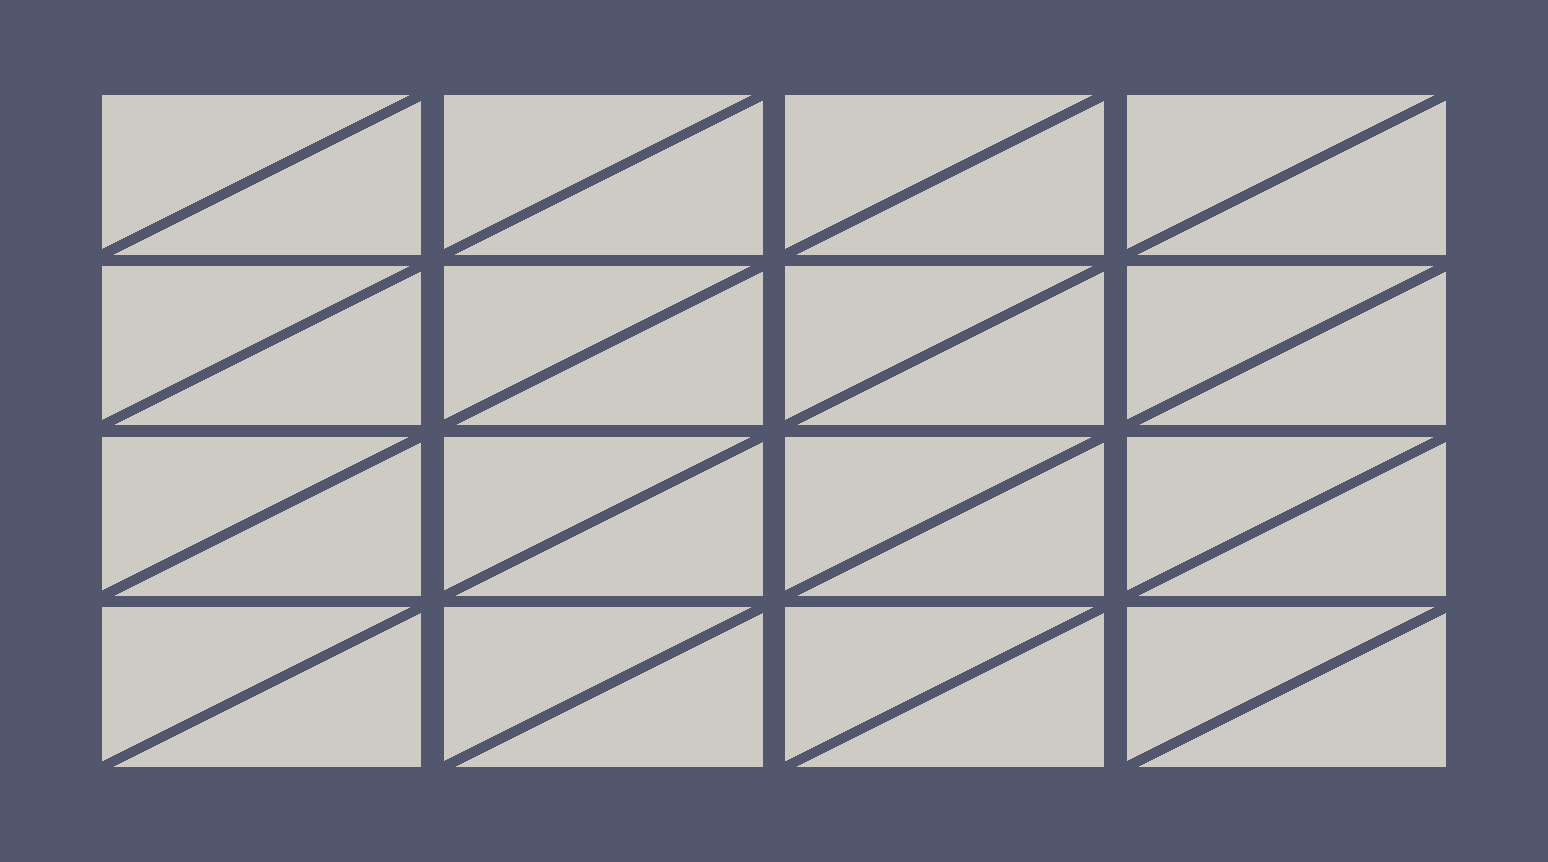
\includegraphics[width=0.5\textwidth]{figures/io/structure2.png}
\end{frame}

\only<article>{\enlargethispage{4ex}}
\subsection{GmshReader}
\label{sec:gmsh}
%-----------------------------------------------------------------------------

\begin{frame}[fragile]
\frametitle{GmshReader}
In DUNE there is a mesh reader interface, which can
read meshes generated with Gmsh (available at \url{http://www.geuz.org/gmsh/}).
\begin{itemize}
\item Can only be used with grid managers that support unstructured grids
  (however, gmsh can generate structured grids, which are stored in an
  unstructured format)
\item Supports simplex grids in 2D and 3D
\item Gmsh can use geometries from CAD programs
\item Gmsh supports a quadratic boundary approximation, which is translated into
boundary segments by the reader.
\end{itemize}
\end{frame}

\begin{frame}[fragile]
\frametitle{An easy GmshReader Example}
\begin{lstlisting}[basicstyle=\scriptsize\ttfamily]
#include<dune/grid/uggrid.hh>
#include<dune/grid/io/file/gmshreader.hh>

typedef Dune::UGGrid<2> GridType;
auto grid = Dune::GmshReader<GridType>::read(mshfile);
\end{lstlisting}
\begin{center}
  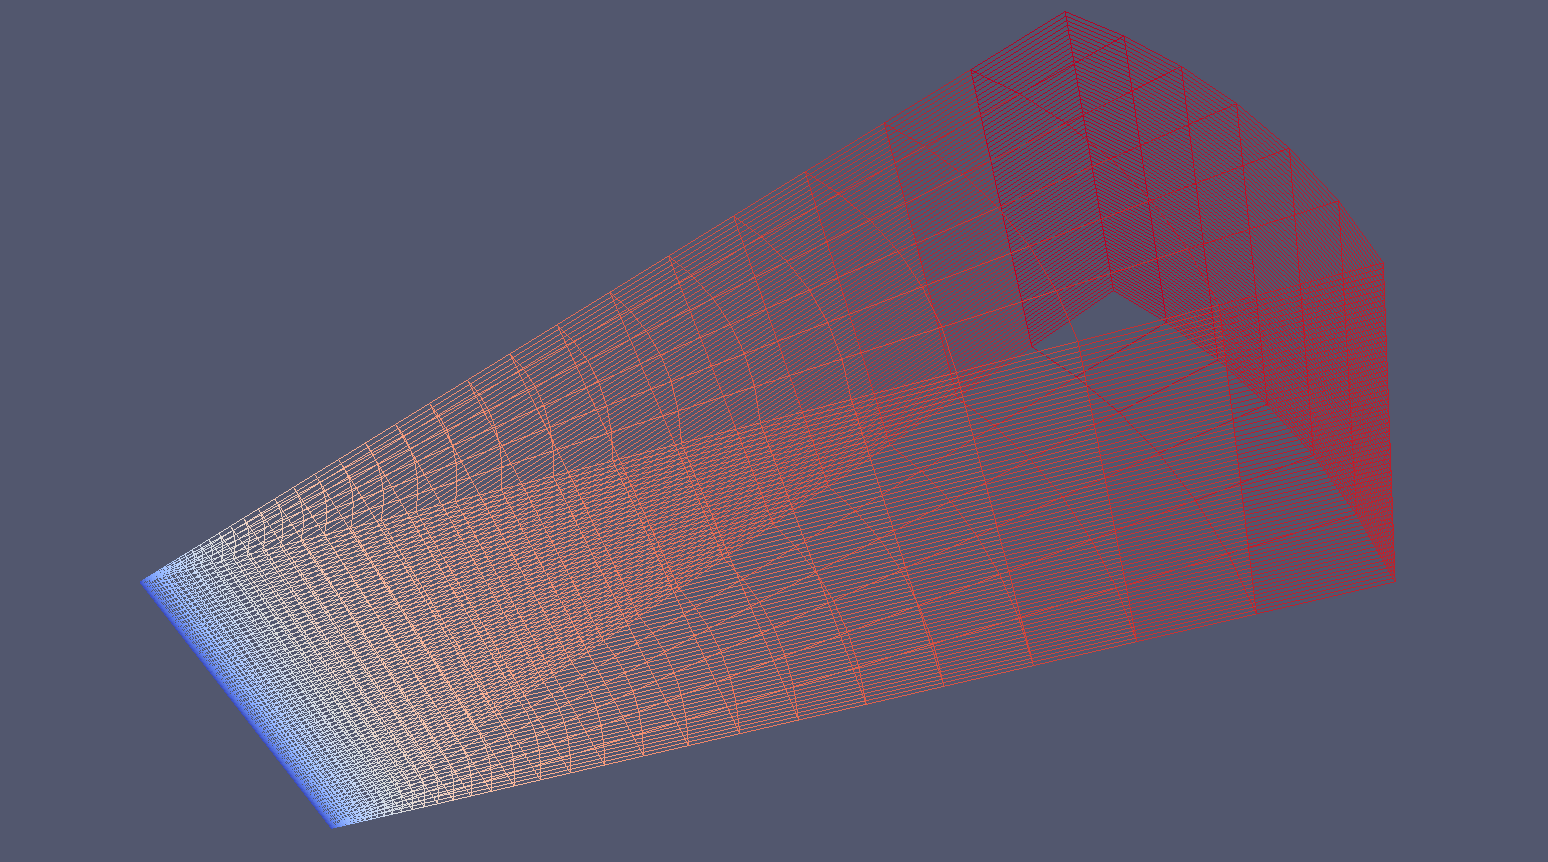
\includegraphics[width=.8\textwidth]{figures/io/easygmsh.png}
\end{center}
\end{frame}

\begin{frame}[fragile]
\frametitle{Attaching data to the grid in gmsh}

GMSH allows you to define physical entities for cells and boundary segments.
The \lstinline!GmshReader! can read those when parsing the msh file and store
them in a \lstinline!std::vector<int>!. The user takes responsibility of those
data structures.
\begin{lstlisting}[basicstyle=\scriptsize\ttfamily]
#include<dune/grid/uggrid.hh>
#include<dune/grid/io/file/gmshreader.hh>

typedef Dune::UGGrid<2> GridType;

std::vector<int> boundaryPhysicalEntities;
std::vector<int> elementPhysicalEntities;

auto grid = Dune::GmshReader<GridType>::
    read(mshfile, boundaryPhysicalEntities, elementPhysicalEntities);
);
\end{lstlisting}
\end{frame}

\subsection{Tensor Product Grid}

\begin{frame}[fragile]
 \frametitle{What is a tensor product grid?}
 A tensor product grid is a special kind of a non-equidistant structured cube grid.
 For each direction $i\in\{ 0,\dots ,d-1\}$ we define a monotonuous sequence of
 coordinates:
 \begin{displaymath}
  \left(x^i_j\right)_{j=0}^{N_i}
 \end{displaymath}
 From those coordinates we define the set of grid vertices $V$ as the tensor product
 of those coordinate sequences:
 \begin{displaymath}
   V = \left\{(x^0_{i_0},\dots ,x^{d-1}_{i_{d-1}}) \big| i_j\in \{0,\dots ,N_j\} \forall j=0,\dots ,d-1\right\}
 \end{displaymath}
 The resulting grid has
 \begin{displaymath}
  N = \prod_{i=1}^{d-1}N_i
 \end{displaymath}
 cells.
\end{frame}


\begin{frame}
 \frametitle{Tensorproduct grids in simulations}

 Tensorgrids combine the performance advantages of a structured grid with
 an unstructured grids capability to have different resolutions in different
 parts of the domain.
 \begin{center}
  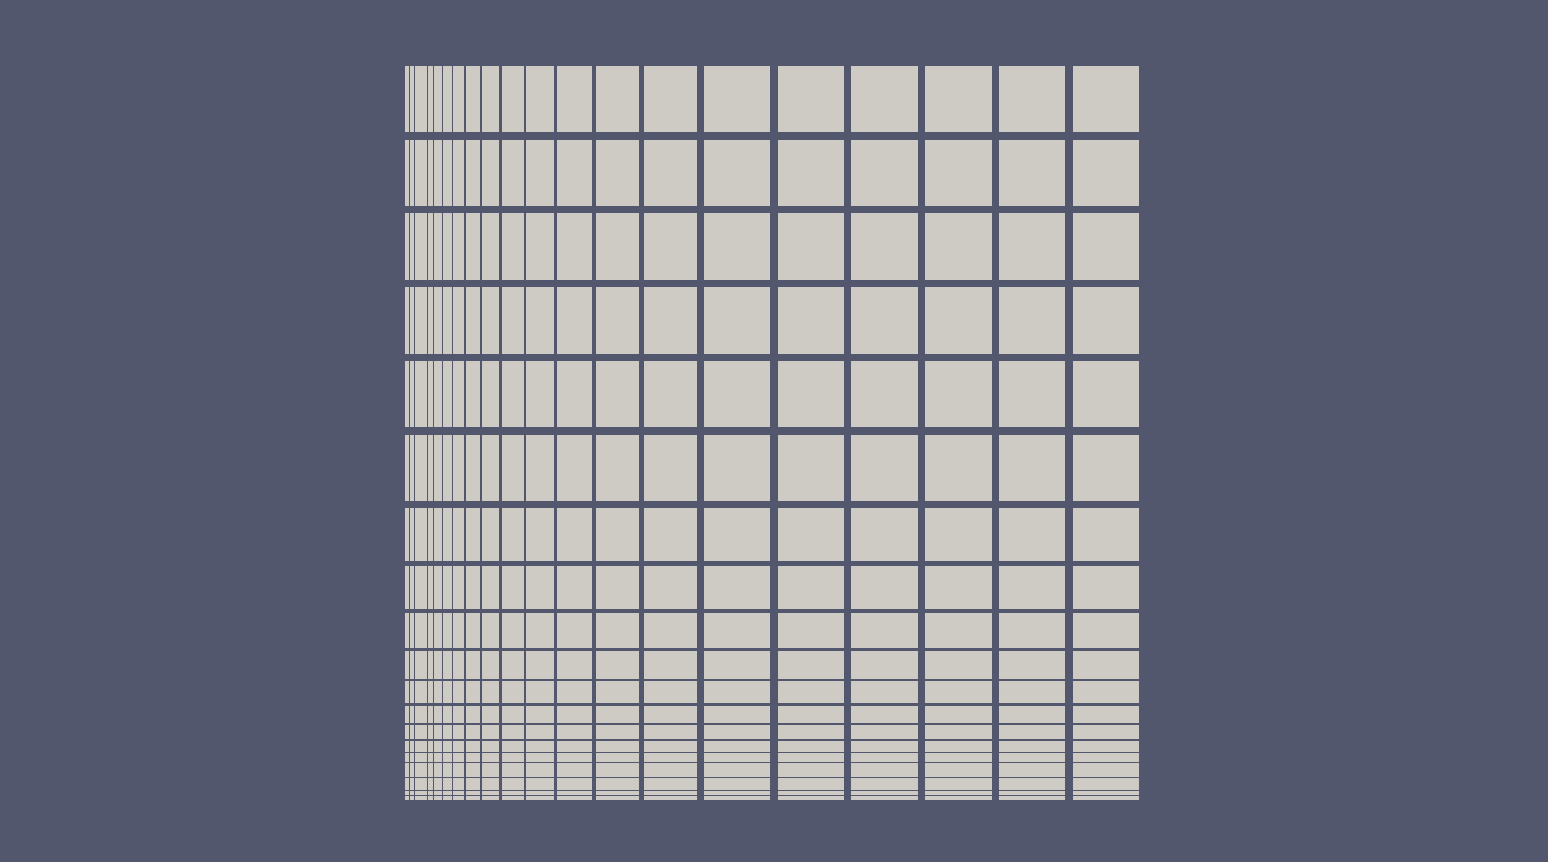
\includegraphics[width=.6\textwidth]{figures/io/tensorprod.png}
 \end{center}
\end{frame}

\begin{frame}
 \frametitle{TensorGridFactory}

 \lstinline!YaspGrid! provides a natural implementation of a tensor product grid.
 The coordinate sequences may be provided manually through \lstinline!std::vector<ctype>!.
 \lstinline!TensorGridFactory! provides convenient methods to fill such coordinate sequences:
 \begin{itemize}
  \item \lstinline!void setStart(int d, ctype value)!
  \item \lstinline!void fillIntervals(int d, int n, ctype h)!
  \item \lstinline!void fillRange(int d, int n, ctype end)!
  \item \lstinline!void geometricFillIntervals(int d, int n, ctype ratio, ctype h0)!
  \item \lstinline!void geometricFillRange(int d, int n, ctype end, ctype h)!
  \item ...
 \end{itemize}

 The TensorGridFactory is compatible with all unstructured grid managers.
\end{frame}

\section{Visualization with VTK}
%-----------------------------------------------------------------------------

\begin{frame}[fragile]
\frametitle{Visualization}

\begin{columns}[b]
\begin{column}{0.5\textwidth}
\begin{itemize}
\item DUNE uses Paraview as a visualization program.
\item Paraview uses the VTK (Visualization Toolkit) file format.
\item Paraview can be obtained for free at \url{http://www.paraview.org}
\end{itemize}
\end{column}
\begin{column}{0.5\textwidth}
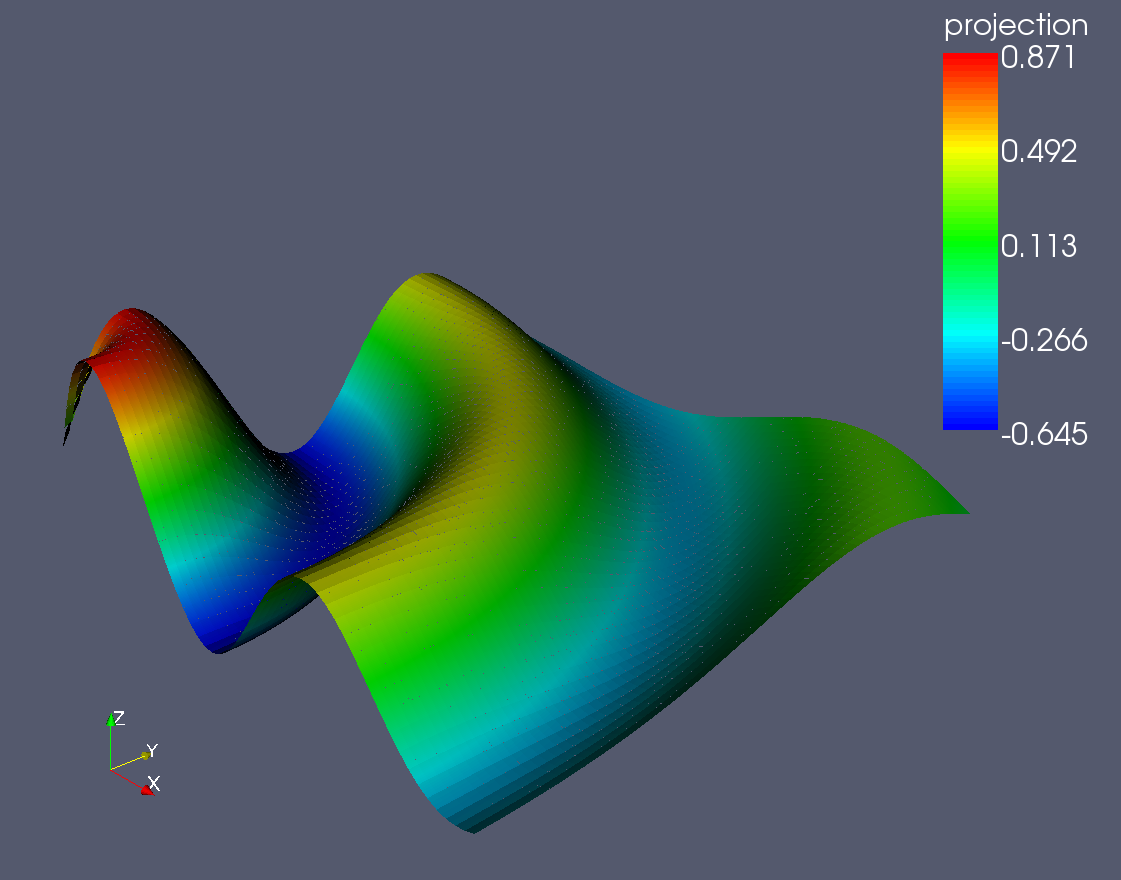
\includegraphics[width=\textwidth]{figures/io/visualisation.png}
\end{column}
\end{columns}

\end{frame}

%-----------------------------------------------------------------------------

\begin{frame}[fragile]
\frametitle{VTKWriter}
\begin{itemize}
\item To use the VTK-writer you have to
  \lstinline!#include<dune/grid/io/file/vtk/vtkwriter.hh>!\\
\item There are two different ways to use the VTKWriter:
\begin{enumerate}
\item Pass the data as a vector to the methods \lstinline!addCellData! or
  \lstinline!addVertexData!.\\
  \structure{This is especially useful if your scheme already stores the
    solution in such a vector, i.e.\ cell- or vertex-centered Finite-Volume
    schemes.}
\item Define your own VTKFunction and pass it to \lstinline!addCellData! or
  \lstinline!addVertexData! as appropriate.\\
  \structure{This is the more general approach and usually done for
    Finite-Element or DG schemes.}
\end{enumerate}
\item After attaching zero or more data fields the data file(s) can be written
  with the \lstinline!write! method of the VTKWriter.
\end{itemize}
\end{frame}


\begin{frame}[fragile]
\frametitle{VTK-Export - Elementdata}
\lstinputlisting[basicstyle=\scriptsize\ttfamily]{src_samples/io/vtkexport-elements.cc}
\end{frame}

\begin{frame}[allowframebreaks]
\frametitle{VTK-Export - Vertexdata}
  \lstinputlisting[basicstyle=\scriptsize\ttfamily]{src_samples/io/vtkexport-vertices.cc}
\end{frame}


%-----------------------------------------------------------------------------

\begin{frame}[fragile]
\frametitle{Defining a VTKFunction}
An output field can also be created by defining a VTKFunction object,
e.g.\ \lstinline!MyVTKFunction<GridView>!.
\begin{itemize}
\item It must be derived from
\lstinline!Dune::VTKWriter<GridView>::VTKFunction!
\item It has to provide the following functions:
\begin{itemize}
  \lstset{numbers=none}
\item the number of components (i.e. whether the plot value is scalar or
  e.g.\ a velocity vector):
  \begin{lstlisting}[numbers=none,basicstyle=\scriptsize\ttfamily]
virtual int ncomps() const;
  \end{lstlisting}
\item a function returning the value of the plot function for the component
  \lstinline!comp! at position \lstinline!xi! in entity \lstinline!e!:
  \begin{lstlisting}[numbers=none,basicstyle=\scriptsize\ttfamily]
virtual double evaluate(int comp, const Entity& e,
    const Dune::FieldVector<ctype,Grid::dimension>& xi
    ) const;
  \end{lstlisting}
\item the name of the plot function to be written in the VTK-file:
  \begin{lstlisting}[numbers=none,basicstyle=\scriptsize\ttfamily]
virtual std::string name() const;
  \end{lstlisting}
\end{itemize}
\end{itemize}
\end{frame}

%-----------------------------------------------------------------------------

\begin{frame}[allowframebreaks=1.0]
\frametitle{VTK-Export - VTKFunction}
  \only<presentation>{
    \lstinputlisting[lastline=22,basicstyle=\scriptsize\ttfamily]{src_samples/io/vtkexport-vtkfunction.cc}
    \lstinputlisting[firstline=24,firstnumber=24,basicstyle=\scriptsize\ttfamily]{src_samples/io/vtkexport-vtkfunction.cc}
  }
  \only<article>{
    \lstinputlisting{src_samples/io/vtkexport-vtkfunction.cc}
  }
\end{frame}

%-----------------------------------------------------------------------------

\only<article>{\newpage}

\begin{frame}[allowframebreaks,fragile]
\frametitle{VTKWriter vs.\ SubsamplingVTKWriter}

\only<presentation>{
\begin{columns}[t]
\begin{column}{0.5\textwidth}
\centering
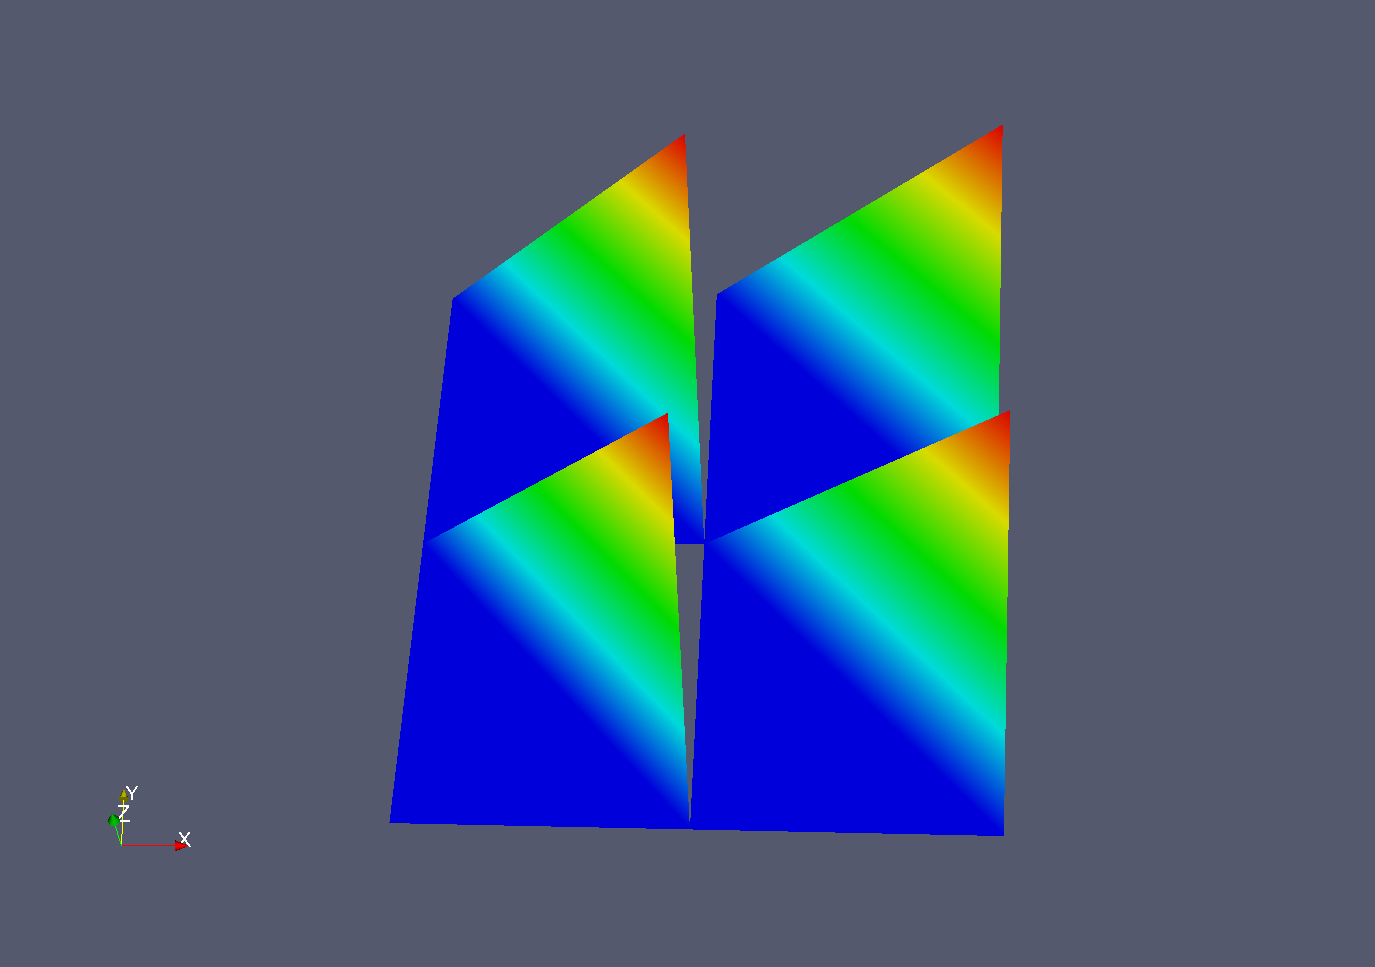
\includegraphics[width=\textwidth]{figures/io/vtkwriter.png}\\
Regular VTKWriter
\end{column}
\begin{column}{0.5\textwidth}
\centering
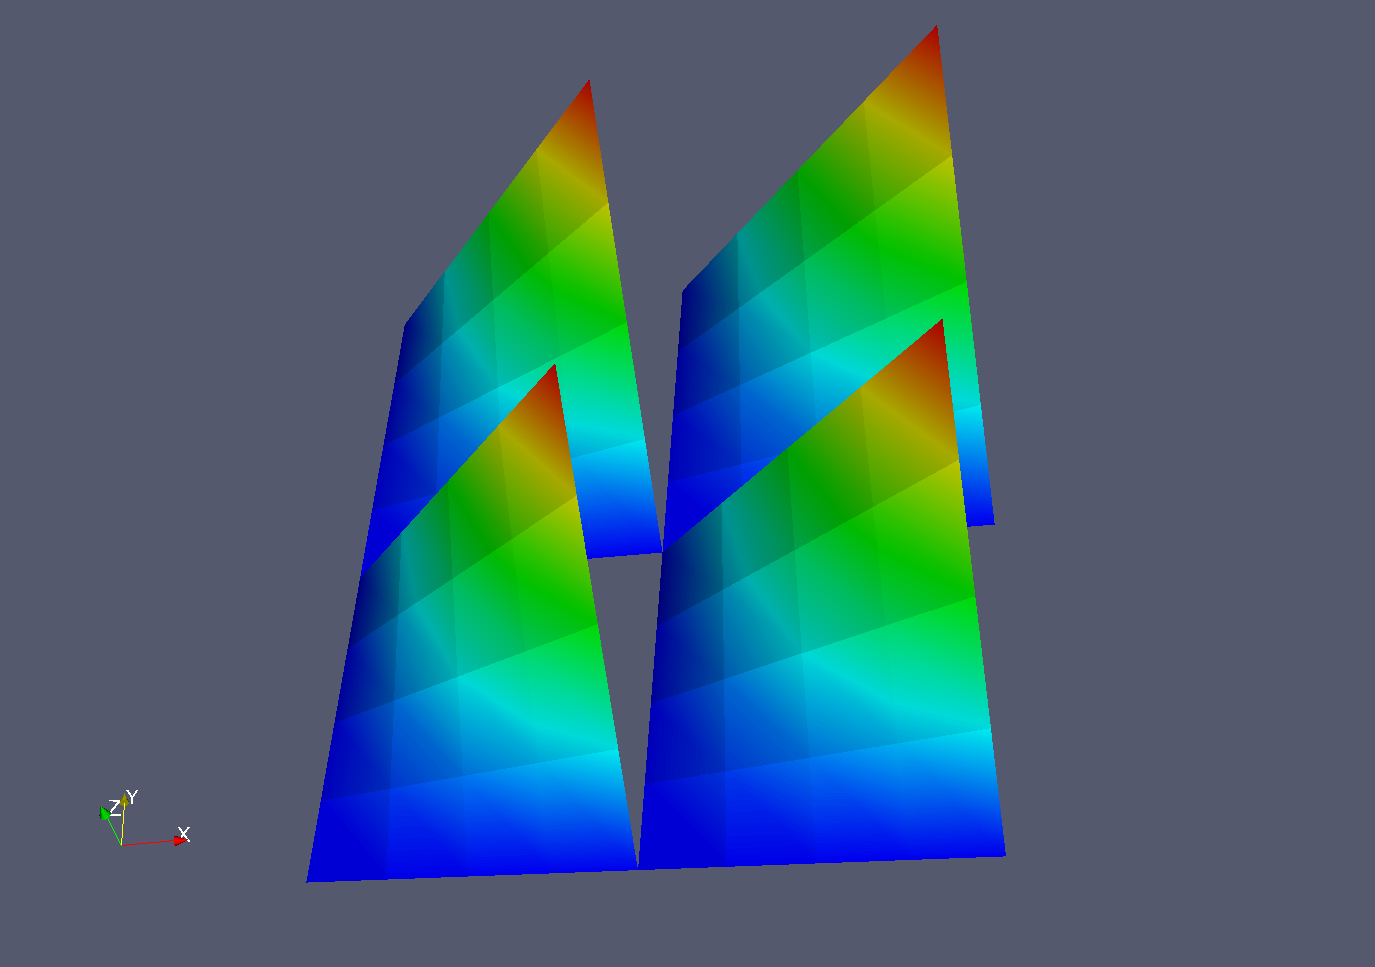
\includegraphics[width=\textwidth]{figures/io/subsamplingvtkwriter.png}\\
SubsamplingVTKWriter\\
% {\scriptsize(written by the previous program)}
\end{column}
\end{columns}\vspace\baselineskip
}

\framebreak

To visualize more complex functions (higher order or mesh elements other than
triangles or tetrahedra), a subsampling VTKWriter is needed.

Necessary Changes:

\begin{lstlisting}[numbers=none,basicstyle=\scriptsize\ttfamily]
#include<dune/grid/io/file/vtk/subsamplingvtkwriter.hh>
Dune::SubsamplingVTKWriter<GridView> vtkwriter(gv, Dune::RefinementIntervals(2));
\end{lstlisting}

This creates a subsampling VTKWriter and tells it to generate 2-times
subrefined output. %
This happens ``virtually'', i.e.\ without modifying the grid.
\end{frame}

\only<article>{
  \begin{figure}[H]
    \centering
    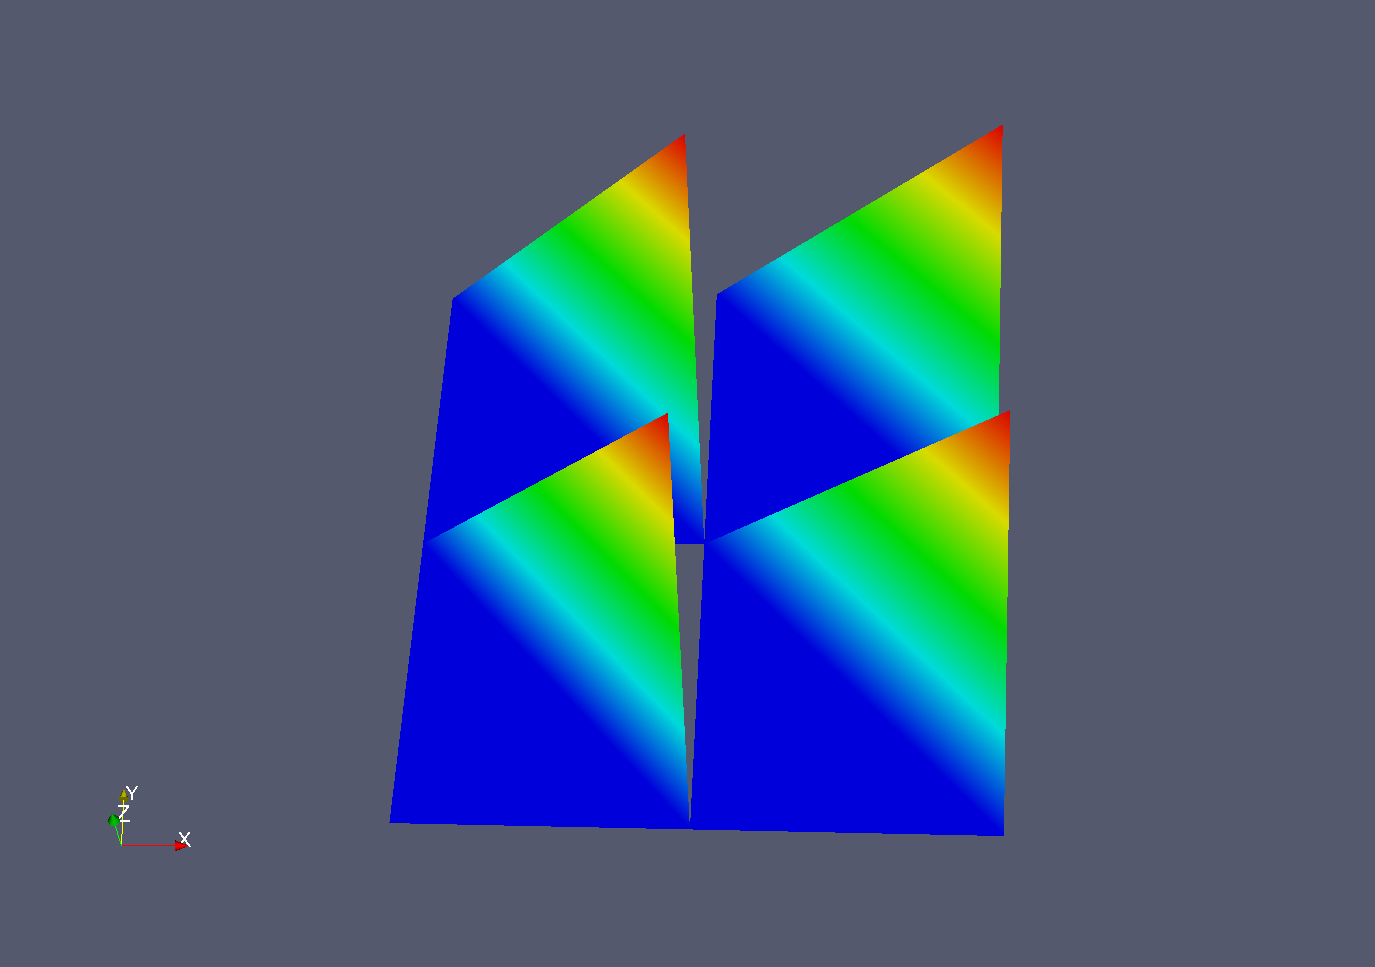
\includegraphics[width=0.48\textwidth]{figures/io/vtkwriter.png}\hfill
    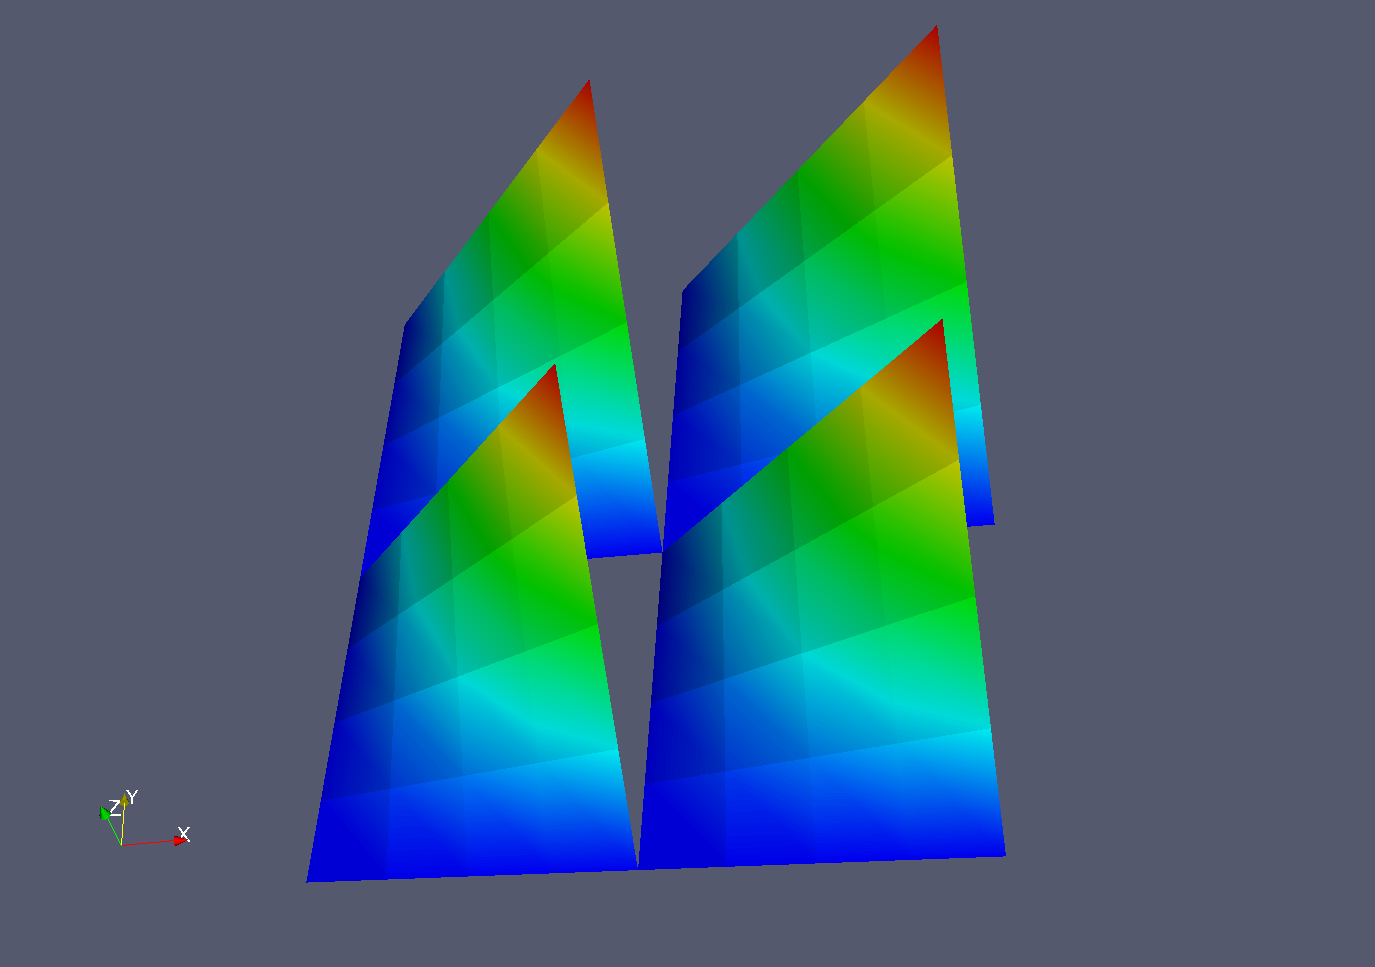
\includegraphics[width=0.48\textwidth]{figures/io/subsamplingvtkwriter.png}\\
    \caption{Visualization of $f(x_l,y_l)=x_ly_l$ using the ordinary
      (left) and the subsampling VTKWriter (right).  The subscript $l$ denotes
    element-local coordinates.}
  \end{figure}
}

\end{document}

%%% Local Variables:
%%% mode: latex
%%% TeX-master: "lectures-beamer"
%%% TeX-PDF-mode: t
%%% End:
